\documentclass[letterpaper]{article} % DO NOT CHANGE THIS
\usepackage[submission]{aaai2027} % DO NOT CHANGE THIS
% The serif, sans-serif, and monospaced fonts are loaded automatically by
% aaai2027.sty (newtxtext, helvet, courier). DO NOT add \usepackage{times},
% \usepackage{helvet}, \usepackage{courier}, or any other font package.
\usepackage[hyphens]{url} % DO NOT CHANGE THIS
\usepackage{graphicx} % DO NOT CHANGE THIS
\urlstyle{rm} % DO NOT CHANGE THIS
\def\UrlFont{\rm} % DO NOT CHANGE THIS
\usepackage{natbib} % DO NOT CHANGE THIS AND DO NOT ADD ANY OPTIONS TO IT
\usepackage{caption} % DO NOT CHANGE THIS AND DO NOT ADD ANY OPTIONS TO IT
\frenchspacing % DO NOT CHANGE THIS

% --- Math / theorems / tables (compatible with aaai2027.sty) ---
\usepackage{amsmath,amssymb,amsthm}
\theoremstyle{plain}
\newtheorem{theorem}{Theorem}
\newtheorem{proposition}{Proposition}
\usepackage{booktabs}

\pdfinfo{
/TemplateVersion (2027.1)
}

\newcommand{\wcrit}{w_{\mathrm{crit}}}
\newcommand{\PT}{\mathrm{PT}}

\setcounter{secnumdepth}{0}

\title{Measuring Coordination-Collapse Boundaries in Reward-Mixed Cooperative MARL}

\author{
  Anonymous Submission
}
\affiliations{
  Paper under double-blind review
}

\begin{document}

\maketitle

% =======================================================================
\begin{abstract}
Cooperative multi-agent reinforcement learning (MARL) can collapse into degenerate
\emph{lazy-agent} policies when each agent's local reward overwhelms the team signal. We ask not
whether centralization helps but \emph{where}: at what critical team-reward fraction $\wcrit$ a
trained population crosses into a pre-specified collapse region. We measure this boundary by
sweeping the local-to-team reward mixture $w$, fitting $P(\mathrm{collapse}\mid w)$, and reporting
$\wcrit$ with bootstrap confidence intervals; on our primary supply-chain testbed
$\wcrit=0.666$ $[0.635,0.694]$. Using the instrument, we then test a loss-averse reward transform,
which weights losses more heavily than equal gains, applied after reward blending. Loss aversion
shifts $\wcrit$ rightward, so agents need more team reward to coordinate; the direction replicates
across four environment-algorithm combinations, while longer training slides the boundary left. At
a moderate setting ($\lambda{=}3$) the full transform moves the boundary $+0.089$ relative to the
linear reward, or $+0.188$ once value-function curvature is separated from loss aversion. On the
supply chain the instrument also exposes scoped secondary findings, including that a single
downstream loss-averse node can nearly set the boundary. The contribution is a protocol for
measuring where a cooperative learning system crosses into collapse, rather than only asserting
that centralization helps.
\end{abstract}

% =======================================================================
\section{Introduction}
\label{sec:intro}

A team of learning agents can fail even when the task has a good cooperative solution: instead of
learning complementary behavior, each agent settles into a locally safe, low-cooperation policy,
and the team lands in a stable, useless equilibrium. We call this \emph{coordination collapse};
in the MARL literature its endpoint is the \emph{lazy-agent}
policy~\citep{liu2023lazy,peng2023curo}, and the underlying private-versus-collective conflict is
the one studied in sequential social dilemmas~\citep{leibo2017multi}. We study this failure through
a \emph{reward-centralization} dial: within each reward-mixing sweep, agent $i$ is trained on the
blended scalar $x_i(w)=(1-w)\,r_i^{\mathrm{local}}+w\,r^{\mathrm{global}}$, $w\in[0,1]$, so at
$w{=}0$ the learner sees only its own local reward and at $w{=}1$ only the team reward. Turn $w$
down and an agent's private performance drowns out its contribution; cooperating earns no
learnable signal and the lazy policy wins. That decentralized reward shaping cannot match
centralized training is broadly accepted~\citep{dmarl2025}, and lazy-agent and credit-assignment
work~\citep{liu2023lazy,peng2023curo,sunehag2018vdn,rashid2018qmix,foerster2018counterfactual}
mitigates the pathology; what none of it supplies is the \emph{location}. The closest phase-diagram
studies place their critical points on \emph{environmental}~\citep{yamaguchi2025} or
opinion-dynamics~\citep{capannoli2026phase} axes rather than reward structure, and none estimates a
confidence-intervalled crossing in reward-centralization space for gradient-trained cooperative
policies. Our central question is therefore twofold: does coordination collapse admit a
\emph{measurable} critical centralization threshold $\wcrit$, and do prospect-theoretic reward
transforms systematically shift it? The first is a measurement problem (the paper's primary
contribution); the second is a question the instrument then makes answerable.

Pinning down this number for a given training setup matters because reward design is not neutral.
$\wcrit$ is not universal: it is a measured property of an environment, learner, training horizon,
and collapse label, and it tells a designer where their own system crosses into collapse. Applying
the instrument requires a reward-mixing dial and a learner that can coordinate at high
centralization; a third condition is narrower and empirical, in that on the supply-chain base-stock
control a coarse action discretization erases the boundary, whereas action-discrete environments
such as MPE still exhibit one (see the scope condition below). We estimate $\wcrit$ in four
environment-algorithm combinations: a six-node inventory network under PPO and under MAPPO, and
Cooperative Navigation (MPE) and Level-Based Foraging (LBF) under MAPPO. The inventory network is a
branching directed-flow graph, which later lets us ask \emph{which} node's reward design sets the
boundary. Because the boundary is finite-horizon, we re-measure it at several horizons; the rate at which
extra training substitutes for centralization is itself one of the quantities we report. More broadly, any cooperative learning system that blends local and team rewards, or trains
with preference-shaped objectives and human-motivated reward
transforms~\citep{ethayarajh2024kto,lalmohammed2025}, faces the same design question. We use
prospect theory only as a controlled reward-transform family, not as a
psychological claim: after local and team rewards are blended, the scalar is transformed with
value-function curvature and loss aversion, the asymmetry in which a loss looms larger than an
equal gain~\citep{kahneman1979,tversky1992}, while the learner, architecture, optimizer, and
evaluation label are unchanged. The experimental question is then clean: does changing the scalar
training signal move the collapse boundary?

We build the instrument before using it. Three design choices make a reading trustworthy: the
collapse label is a behavioral rule scored on evaluation behavior rather than training reward, and
pre-registered on the supply-chain substrate (label, analysis code, and probes committed before
execution); matched policies differ only in the scalar training signal, because the
prospect-theoretic transform is applied after blending, outside the optimizer; and every $\wcrit$ is
reported with a bootstrap confidence interval. ``Phase boundary'' is used only in this operational sense, an empirical crossing in
learning dynamics, not thermodynamic criticality. The contributions are: (i)~a
confidence-intervalled boundary instrument for reward-mixed cooperative MARL; (ii)~a replicated
finding that loss aversion shifts the boundary rightward, so agents require more centralization to
coordinate, with that direction and the finite-horizon slide holding across four
environment-algorithm combinations; and (iii)~a scoped supply-chain analysis, comprising a
sign-level mean-field account, a bounded one-parameter summary of the $\lambda$-sweep, and a
directed-flow finding that a single downstream node's reward design can nearly set the whole team's
boundary. The magnitudes and secondary structure are substrate-specific unless separately
replicated.

% =======================================================================
\section{Related Work}
\label{sec:related}

\paragraph{Coordination collapse and credit assignment.}
Cooperative MARL, studied since independent $Q$-learning on shared
tasks~\citep{tan1993multi,busoniu2008comprehensive}, inherits the lazy-agent and
relative-overgeneralization failures in which agents abandon cooperation for a degenerate
policy~\citep{liu2023lazy,peng2023curo,tampuu2017multiagent}. The standard remedy is centralized
credit assignment under CTDE, a centralized critic or factorized value
function~\citep{lowe2017multi,yu2022surprising,sunehag2018vdn,rashid2018qmix,foerster2018counterfactual,son2019qtran};
related work ties the failure to
decentralized exploration~\citep{weng2026} or shows decentralized shaping cannot match centralized
baselines~\citep{dmarl2025}. This establishes \emph{that} centralization helps and \emph{how} to
implement it; none locates the threshold $\wcrit$ or gives it a confidence interval, the gap we
close, using $w$ as the dial rather than a fixed factorization.

\paragraph{Phase transitions in multi-agent learning.}
Treating collective learning as a dynamical system with critical points has
precedent: \citet{yamaguchi2025} builds a phase diagram for independent Q-learning over
\emph{environmental} axes, and \citet{capannoli2026phase} prove a metastable boundary in opinion
dynamics under a fixed update rule. Mean-field and dynamical-systems analyses derive deterministic
or distributional limits for multi-agent learning: a Fokker--Planck description of $Q$-learning in
large populations~\citep{hu2019meanfield}, the deterministic limit of temporal-difference learning
in stochastic games~\citep{barfuss2019deterministic}, and convergence in random
networks~\citep{hussain2025convergence}. We borrow the phase-diagram measurement style but differ in
object: ours is a \emph{reward-structure} threshold with confidence intervals that a
prospect-theoretic reward transform moves, and we use the mean-field machinery only for a
sign-level account.

\paragraph{Behavioral preferences in cooperative AI.}
Human preference structure has entered collective learning only narrowly.
\citet{hughes2018inequity} show inequity aversion improves cooperation within the cooperative-AI
agenda~\citep{dafoe2020open,hammond2025multiagent,barfuss2020caring}, and loss aversion is now a
training objective at scale: KTO aligns language models with a Kahneman--Tversky value function
carrying an explicit loss-aversion coefficient~\citep{ethayarajh2024kto}. Risk-sensitive RL
optimizes tail outcomes~\citep{qiu2021rmix,xie2023riskq,prashanth2014cvar,tamar2015optimizing},
distinct from loss aversion, a reference-point asymmetry, and prospect theory has entered
single-agent RL with known calibration
concerns~\citep{prashanth2016cumulative,rabin2000risk,tversky1992}. In the multi-agent setting,
\citet{mengesha2025} find loss aversion has a \emph{non-monotone} effect on equilibrium selection in
an evolutionary model with quantal response, and \citet{lalmohammed2025} bring CPT into cooperative
MARL but fold it into the actor--critic update, so its value and probability-weighting components
vary jointly with the optimizer. We differ at the level of \emph{apparatus}: rather than proposing
another behavioral model, we build a measured boundary and use it as a common instrument; the
prospect-theoretic reward-transform study is its first application, not the instrument's whole
contribution.

% =======================================================================
\section{Preliminaries and Method}
\label{sec:method}

We study \emph{reward-mixed} cooperative MARL: settings in which $N$ agents share an environment
and each learner's scalar training reward is a blend of a local term and a team term. The learners
range from independent policy gradients to centralized training with decentralized execution
(CTDE)~\citep{lowe2017multi}; our primary supply-chain learner is independent PPO, while the
transfer settings use a centralized critic. The restriction to a blended reward is deliberate: it
yields a controllable reward-design axis $w$. For agent $i$, the blended scalar is
$x_i(w)=(1-w)\,r_i^{\mathrm{local}}+w\,r^{\mathrm{global}}$, $w\in[0,1]$, so $w$ is not an optimizer
hyperparameter but a structural property of the reward design. We do not rescale
$r_i^{\mathrm{local}}$ or $r^{\mathrm{global}}$ separately at each $w$; both remain in the
environment's native units, so a given $w$ means the same local/team mixture in every condition
rather than hiding a per-condition normalization. When $w$ is small, an agent can protect its local
reward while contributing little to the team; in tasks with local--global conflict this makes the
low-cooperation policy easier to learn than the coordinated one~\citep{liu2023lazy,peng2023curo}.
Unless stated otherwise, each experiment varies one factor at a time, holding the learner,
environment, horizon, transform parameters, and collapse label fixed while a single named sweep
moves.

The boundary estimate follows four steps: fix the environment, learner, horizon, and collapse
label; train matched policies across a grid of $w$; label each run from pre-specified
\emph{evaluation} behavior, not training reward; and fit a monotone binary model
$P(\mathrm{collapse}\mid w)$, reporting the midpoint $\wcrit$ with bootstrap confidence intervals.

The reward transform is prospect-theoretic in value-function form. For the blended scalar
$x=(1-w)r_i^{\mathrm{local}}+w r^{\mathrm{global}}$, with zero as the reference point for gains
and losses, we use $v(x)=x^\alpha$ for $x\ge0$ and $-\lambda(-x)^\beta$ for $x<0$. The exponents
$\alpha,\beta\in(0,1]$ control \emph{curvature}: below one the transform is concave, so a reward of
$100$ is worth less than twice a reward of $50$ and large outcomes are compressed toward small ones.
The multiplier $\lambda>1$ is separate: it scales the entire loss branch, so a loss of magnitude
$x$ counts $\lambda$ times as much as a gain of $x$ (\emph{loss aversion}), and
$\alpha{=}\beta{=}1,\lambda{=}1$ leaves the reward unchanged, $v(x)=x$. Because curvature is present
in every loss-aversion condition, it must be measured on its own, or its effect is silently folded
into the $\lambda$ shift; this is why we run a curvature-only baseline. Full cumulative prospect
theory also reweights outcome probabilities; we omit that channel, so the only thing that varies
between matched runs is the scalar value transform. We apply it after blending,
\begin{equation}
 r_i^{\PT}=v\!\left((1-w)\,r_i^{\mathrm{local}}+w\,r^{\mathrm{global}}\right),
 \label{eq:reward}
\end{equation}
which keeps the optimizer and architecture bit-identical across matched conditions. This is the
difference from \citet{lalmohammed2025}, who embed CPT \emph{inside} the actor--critic update; that
is appropriate for their aims but varies the value transform, probability weighting, and the
optimizer together. A measured shift is therefore attributed to the transform channel under study,
while recognizing that reward scale, variance, and advantage shape are part of that channel.

A \emph{collapse label} is a pre-specified binary evaluation rule marking runs whose behavior lies
inside a low-cooperation region, scored on held-out evaluation episodes rather than training reward.
In the supply chain, collapse is $\mathbf{1}[\bar S<10\wedge\bar\pi\le-127.1]$, with $\bar S$ the
mean base-stock and $\bar\pi$ the mean profit over deterministic evaluation; this corresponds to
low/no ordering with poor profit. Collapsed runs pile up at the lazy attractor's deterministic
profit floor ($\approx-128$), so the profit clause is effectively a redundancy check on
$\bar S<10$ rather than a tuned cutoff. In MPE (Cooperative Navigation), collapse is landmark
occupancy below $\theta=0.144$, i.e.\ agents cluster rather than cover landmarks; in LBF
(Level-Based Foraging), collapse is mean team return below $\theta=0.626$ (the calibrated
collapsed-versus-coordinated midpoint), i.e.\ agents fail to cooperatively load food.\footnote{The supply-chain
label, analysis code, and mechanism probes---including two probes that later returned negative
results (Supplement)---were committed before execution; the anonymized bundle freezes them, and the
de-anonymized commit hash is released on acceptance.} Threshold robustness holds among estimable
$\pm20\%$ variants (max $\Delta\wcrit=0.015$; Supplement).

For each condition we fit a logistic model $P(\mathrm{collapse}\mid w)=\sigma(b_0+b_1 w)$, where
$b_0$ is the intercept and $b_1$ the slope in $w$ (negative, since collapse falls as $w$ rises), and
report $\wcrit=-b_0/b_1$, the $w$ at which fitted collapse probability is $0.5$. Confidence intervals
are percentile bootstrap over runs~\citep{efron1993bootstrap} ($2{,}000$ resamples). When collapse is near-perfectly separated
across adjacent $w$ (steep high-$\lambda$ cells), the ordinary logistic slope diverges, so those
cells use Firth's bias-reduced logistic regression~\citep{firth1993}, whose $\wcrit$ agrees with the
bootstrap estimate to within $0.019$ at every $\lambda$. The transition width is the fitted 10--90
width, $\Delta w=(\mathrm{logit}(0.9)-\mathrm{logit}(0.1))/|b_1|$, reported alongside location. The
decomposition compares three conditions with identical environment and optimizer: the
\textbf{linear baseline} ($\alpha{=}\beta{=}1,\lambda{=}1$; no curvature, no loss aversion), the
\textbf{curvature baseline} ($\alpha{=}\beta{=}0.88,\lambda{=}1$), and \textbf{loss-aversion
conditions} ($\alpha{=}\beta{=}0.88,\lambda>1$). The primary substrate is
\texttt{NetworkManagement-v1}~\citep{hubbs2020orgym}, a six-node multi-echelon inventory
network~\citep{oroojlooyjadid2022,gijsbrechts2022,marlim2023}; transfer environments are MPE
Cooperative Navigation~\citep{lowe2017multi} and Level-Based Foraging~\citep{christianos2020shared}.
We choose the supply chain as primary because it exposes a directed-flow coordination failure and
supports the minority-topology analysis; the instrument itself only requires a reward-mixing dial
and a pre-specified collapse label. Supply-chain agents run independent PPO~\citep{schulman2017ppo}
via Stable-Baselines3~\citep{raffin2021sb3}; MPE, LBF, and the cross-algorithm supply-chain control
use MAPPO---PPO with a centralized (joint-state) critic~\citep{yu2022surprising}, implemented on the
same Stable-Baselines3 stack. All environments are wrapped with
PettingZoo/SuperSuit~\citep{terry2021pettingzoo,terry2020supersuit}. Headline $\lambda$ sweeps use
$20$ seeds per $(w,\lambda)$ cell; the full run inventory, including the $450$k/$900$k horizons, the
finer high-$\lambda$ grid, and the entropy ablation, is itemized in the Supplement.
\textbf{Reading guide.} All primary results are measured on the supply chain under PPO; MPE, LBF, and
MAPPO are transfer settings used to test which claims travel, and the claim ledger
(Table~\ref{tab:ledger}) states which is which.

% =======================================================================
\section{The Boundary and Its Reward-Transform Shift}
\label{sec:results}

\paragraph{A sharp boundary exists at fixed training budget.}
At 300k steps on the supply-chain PPO substrate, collapse has a clear boundary in
reward-centralization space: the fitted midpoint is $\wcrit=0.666$ $[0.635,0.694]$. The transition
is sharp rather than a gradual decay: fitted collapse probability rises from 10\% to 90\% over
$\Delta w=0.199$, and a Firth logistic-slope test rejects a flat relationship between $w$ and
collapse ($p=3.2\times10^{-7}$; Figure~\ref{fig:boundary}a). We use 300k as the primary horizon
because the risk-neutral boundary is interior and sharply estimable there; horizon dependence is
measured separately below.

\paragraph{The boundary is finite-horizon and metastable.}
The boundary slides left with the training horizon: across four matched risk-neutral horizons,
$\wcrit=0.822,0.666,0.622,0.573$ at $150\mathrm{k},300\mathrm{k},450\mathrm{k},900\mathrm{k}$
steps, and the slide is \emph{log-linear in $T$}: $\wcrit=2.44-0.138\ln T$ (RMSE $0.027$; all four
CIs of width ${\le}0.073$, the last three ${\le}0.054$; Figure~\ref{fig:boundary}b). This is
consistent with metastable escape (a Kramers-type first-passage picture, developed below): each
doubling of the budget buys a fixed $\approx0.10$ leftward shift, so longer training rescues some
runs that collapse at shorter horizons. An illustrative extrapolation to $2\mathrm{M}$ steps gives
$\wcrit\approx0.44$, but the claim is limited to the measured horizons; the deterministic floor
$\wcrit^0=c/(c+g)$ derived below is treated as lying beneath the measured range. Horizon dependence does not make
$\wcrit$ arbitrary: at any fixed budget it is well-defined, and the slide quantifies the rate at
which extra training substitutes for centralization.

\paragraph{The horizon slide is not a supply-chain artifact.}
Under centralized-critic MAPPO the same slide recurs in both transfer environments: on MPE
$\wcrit$ falls $0.82\to0.68$ as the horizon grows $2\mathrm{M}\to8\mathrm{M}$, and on Level-Based
Foraging $0.33\to0.20$ over $1\mathrm{M}\to4\mathrm{M}$, both with non-overlapping endpoint
intervals. A basin-control experiment checks a simple confound, that runs collapse because their
initial policies start closer to the lazy basin: within each fixed $w$, correlations between
initial and converged base-stock are only small to moderate ($-0.11$ to $-0.38$) and collapsed
versus surviving runs are not separated by their starting base-stock, so initialization is an
unlikely driver of the measured boundary (Supplement).

\paragraph{Loss aversion raises the boundary; curvature lowers it.}
Three measured baselines anchor the comparison, all with identical environment, PPO learner,
collapse label, and 300k horizon: the structural null of the main sweep
($\alpha{=}\beta{=}1,\lambda{=}1$; $\wcrit=0.666$), the same linear condition independently
reproduced at $0.685$ for the decomposition (other null-like numbers are labeled offsets, not
separate baselines), and the curvature baseline
($\alpha{=}\beta{=}0.88,\lambda{=}1$). We fix $\alpha{=}\beta{=}0.88$ because it is the
conventional prospect-theory curvature estimate~\citep{tversky1992}, not a value tuned to the
task; the loss-aversion sweep then varies only $\lambda\in\{1,\dots,7\}$. The boundary rises
monotonically up to estimation noise, $\{0.586,0.715,0.774,0.806,0.825,0.835,0.852\}$, then
saturates near $0.85$ with clear headroom to the $w{=}1$ ceiling, so the plateau is a
reward-transform saturation, not a ceiling artifact (Figure~\ref{fig:decomposition},
Table~\ref{tab:decomposition}); the endpoints are non-overlapping by $0.221$. Curvature alone acts
in the \emph{opposite} direction, \emph{lowering} $\wcrit$ to $0.586$ ($-0.100$ $[-0.172,-0.033]$
vs.\ the linear baseline). This is why we decompose the transform: reported only as a single
``prospect-theoretic'' treatment, the two effects would partially cancel, since on this substrate
curvature makes coordination easier while loss aversion makes it harder.

\paragraph{Two effect sizes answer two questions.}
The sweep gives boundary locations; effect sizes subtract baselines, and the reported size depends
on the comparison (Table~\ref{tab:decomposition}). The \emph{deployment shift} compares a
transformed reward with the linear baseline and is the total change a designer would see when
replacing the linear reward with the full transform: at $\lambda{=}3$, $\wcrit=0.774$ is $+0.089$
over $0.685$; at $\lambda{=}7$, $+0.167$. The \emph{isolated loss-aversion shift} compares the same
conditions with the curvature baseline ($0.586$) and is the cleaner estimate of the $\lambda$
effect, because curvature is present in every sweep condition: $+0.188$ and $+0.266$ respectively.
The two differ by the curvature offset ($-0.100$ against the linear baseline;
Table~\ref{tab:decomposition}). We highlight
$\lambda{=}3$ as a moderate setting near the canonical loss-aversion range and $\lambda{=}7$ as the
sweep's strongest value; the full series appears in Figure~\ref{fig:decomposition} and the
Supplement. Throughout, ``the loss-aversion effect'' means the increment over the curvature
baseline. The full sweep is additionally summarized by a one-parameter saturating law (below) to
RMSE $0.014$, and a finer $w\in\{0.80,0.90\}$ grid tightens the steep $\lambda{\geq}5$ cells to CI
widths $\approx0.03$.

\begin{figure}[t]
 \centering
 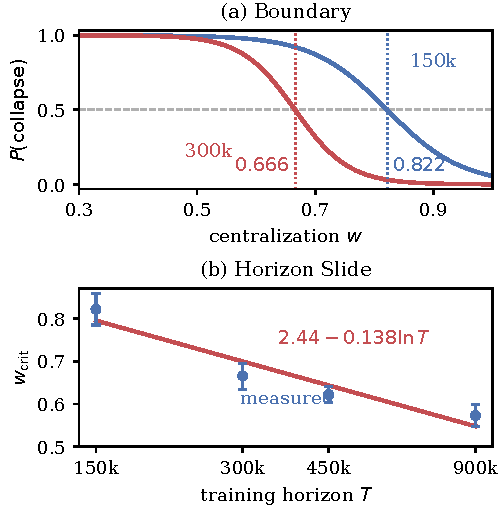
\includegraphics[width=\columnwidth]{Figures/boundary_metastability}
 \caption{Boundary location and horizon slide. (a)~At fixed training budget, collapse changes
  sharply with reward centralization $w$; curves show fitted $P(\mathrm{collapse}\mid w)$ at two
  representative horizons (150k and 300k steps). (b)~All four measured horizons: increasing the
  training horizon shifts $\wcrit$ left, log-linearly in $T$ (RMSE $0.027$; 20 seeds per $w$-cell at
  each horizon), so more training rescues some runs that collapse at shorter horizons.}
 \label{fig:boundary}
\end{figure}

\begin{figure}[t]
 \centering
 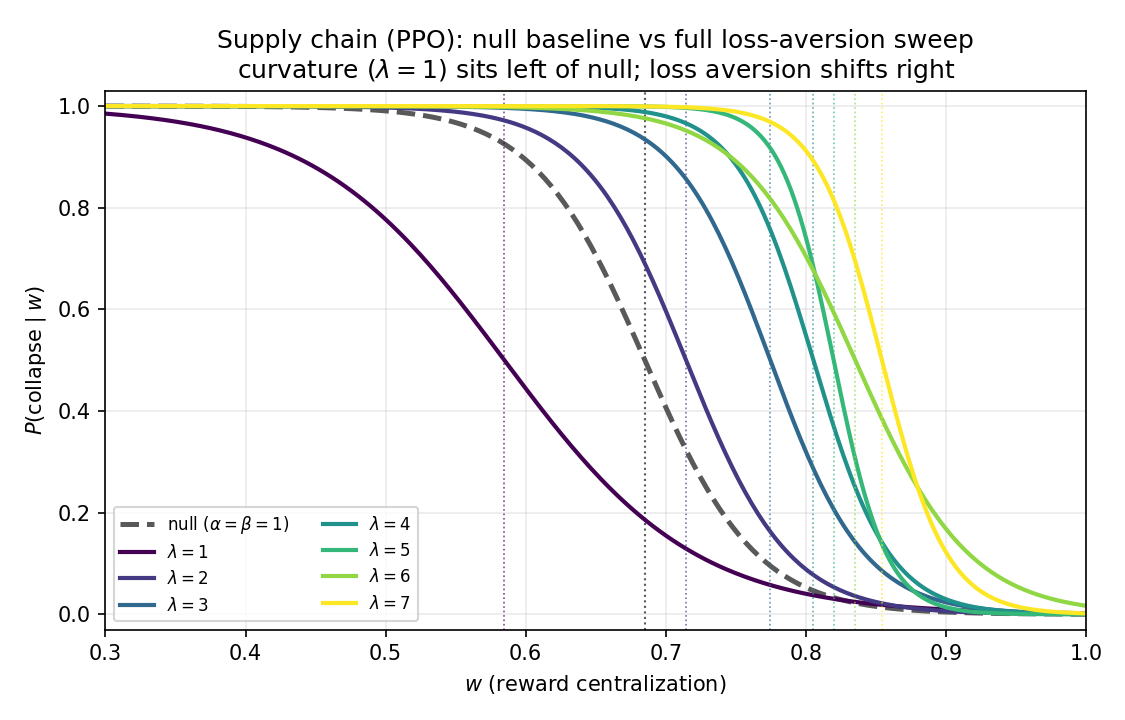
\includegraphics[width=0.92\columnwidth]{Figures/ppo_behavioral_full}
 \caption{Loss aversion raises the collapse boundary (supply chain, PPO). Curves are fitted
  $P(\mathrm{collapse}\mid w)$; dotted lines mark $\wcrit$. Curvature alone
  ($\alpha{=}\beta{=}0.88$, $\lambda{=}1$) shifts the boundary \emph{left} of the linear
  baseline; increasing $\lambda$ then shifts it \emph{right}, saturating near
  $\wcrit\approx0.85$.}
 \label{fig:decomposition}
\end{figure}

\begin{table}[t]
\centering
\caption{Decomposing reward-transform shifts (supply chain, PPO, 300k). ``vs.\ null'' is the
deployment shift against the reproduced linear baseline; ``vs.\ curv.'' is the isolated
loss-aversion shift against the curvature baseline. $\checkmark$ = difference CI excludes zero.}
\label{tab:decomposition}
{\setlength{\tabcolsep}{3pt}\small
\begin{tabular}{lccccc}
\toprule
Condition & $\alpha,\beta$ & $\lambda$ & $\wcrit$ & vs.\ null & vs.\ curv. \\
\midrule
Linear null (rep.) & $1,1$ & 1 & 0.685 & -- & -- \\
Curvature & $0.88,0.88$ & 1 & 0.586 & $-0.100^{\checkmark}$ & -- \\
Loss av. & $0.88,0.88$ & 3 & 0.774 & $+0.089^{\checkmark}$ & $+0.188^{\checkmark}$ \\
Loss av. & $0.88,0.88$ & 7 & 0.852 & $+0.167^{\checkmark}$ & $+0.266^{\checkmark}$ \\
\bottomrule
\end{tabular}}
\end{table}

% =======================================================================
\section{Mechanism: Loss Aversion Lowers Escape SNR}
\label{sec:mechanism}

The measurement above is the paper's contribution; this section adds a scoped mean-field account
of the \emph{sign} of the loss-aversion shift for the primary supply-chain PPO setting. It uses
continuous base-stock actions, the reward-mixing dial $w$, and the observed local--global incentive
conflict, and does not predict the numerical value of $\wcrit$ in closed form. Following mean-field
treatments of multi-agent
learning~\citep{barfuss2019deterministic,hu2019meanfield,hussain2025convergence}, the Supplement
writes the Gaussian policy mean as a diffusion with drift $F$ and update-variance $\Sigma$, so that
escape from the lazy basin to the coordinating basin is a Kramers first-passage
problem~\citep{kramers1940brownian}. The mean escape time scales as
$\tau_{L\to C}\asymp\tau_0\exp(\Delta U)$ with barrier $\Delta U(w,\lambda)$; equating the median
first-passage time to the training budget $T$ gives $\Delta U\approx\ln(T/\tau_0)$. If the barrier
is additionally taken to be approximately linear in $w$ near the crossing---an assumption we adopt
for interpretation but do not derive---this account is consistent with the observed log-linear slide
$\wcrit=a-b\ln T$, which we treat as motivation for the picture rather than a derivation of it. A
run collapses at horizon $T$ when its realized first-passage time exceeds $T$,
so the $50\%$ boundary is where the median first-passage time equals $T$. As a monotone proxy for
the barrier we track the escape signal-to-noise ratio
\begin{equation}
 \mathcal{S}(w,\lambda)=
 \frac{F_{\mathrm{esc}}(w,\lambda)}
 {\sqrt{\Sigma_{\mathrm{esc}}(w,\lambda)}} ,
 \label{eq:snr}
\end{equation}
over the same escape interval, with the finite-horizon boundary at the crossing
$\mathcal{S}(w,\lambda)\approx\kappa_T$, where $\kappa_T$ is a horizon-dependent critical value
(longer horizons require less escape SNR). Increasing $w$ shortens the escape time; increasing loss
aversion lengthens it through the transformed loss-domain signal.

The account also predicts an exploration-noise dissociation rather than uniform movement
everywhere. Injecting entropy is a second SNR-lowering intervention: it raises $\wcrit$ clearly on
LBF (non-overlapping CIs), shifts it in the same direction but within noise on the supply chain
(overlapping CIs), and leaves it flat on MPE, where dense reward and intrinsic exploration dominate
(Figure~\ref{fig:dissociation}). LBF thus confirms the prediction, the supply chain is directionally
consistent, and MPE is a well-powered null. This is indirect support only: two pre-committed probes
reproduced the boundary but did not localize it from drift or basin-flow statistics (Supplement).

\begin{figure}[t]
 \centering
 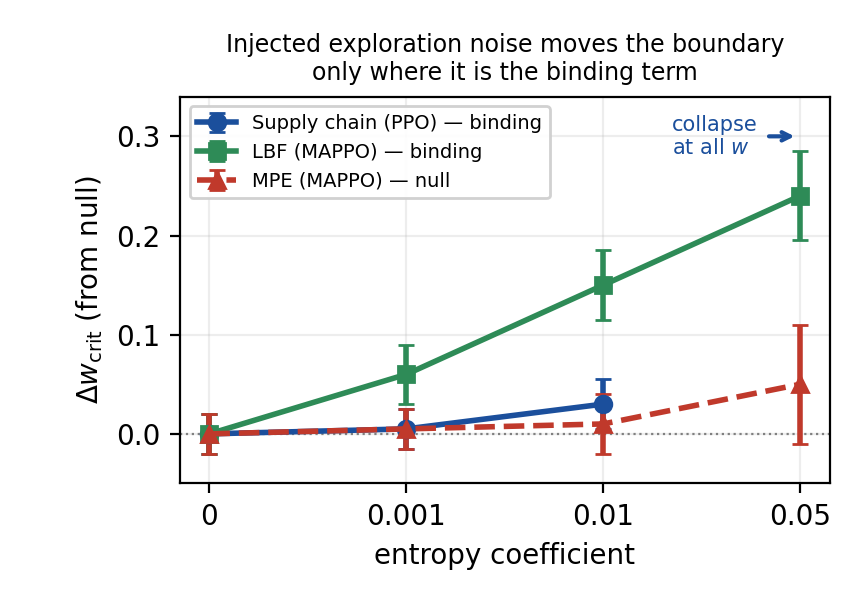
\includegraphics[width=0.82\columnwidth]{Figures/entropy_dissociation.png}
 \caption{Entropy-ablation dissociation. Injected exploration noise raises $\wcrit$ on the
  supply chain (PPO) and LBF (MAPPO), where it is the binding noise term, but leaves the MPE
  boundary flat (overlapping CIs), where dense-reward intrinsic exploration dominates.}
 \label{fig:dissociation}
\end{figure}

The sign result rests on a two-part local premise, and the two parts have different evidential
status. The centralization half, $\partial_w\mathcal{S}>0$, is supported by the measured incentive
signs on the supply chain (Supplement). The loss-aversion half, $\partial_\lambda\mathcal{S}<0$, is
\emph{not} directly measured: our pre-committed probes reproduced the boundary without localizing
it, so we test it only indirectly through the entropy dissociation above, which behaves as a second
SNR-lowering intervention should. The loss-aversion effect may operate through drift, diffusion, or
both, so we state the premise at the SNR level rather than identifying it with drift alone; it is
consistent with the data but not independently verified.

\begin{proposition}[Loss aversion raises the empirical boundary]\label{thm:sign}
Fix a training horizon $T$ and assume, near the boundary: (i)
$\tau_{L\to C}(w,\lambda)=h(\mathcal{S}(w,\lambda))$ with $h,\mathcal{S}$ continuously
differentiable and $h'<0$; (ii) $\partial_w\mathcal{S}>0$ and $\partial_\lambda\mathcal{S}<0$;
(iii) for each $\lambda$ a unique interior $\wcrit^{\mathrm{Emp}}(\lambda)$ solves
$\tau_{L\to C}(w,\lambda)=T$. Then $\mathrm{d}\wcrit^{\mathrm{Emp}}/\mathrm{d}\lambda>0$.
\end{proposition}
\begin{proof}
By (i)--(ii), $\partial_w\tau_{L\to C}=h'(\mathcal{S})\,\partial_w\mathcal{S}<0$ and
$\partial_\lambda\tau_{L\to C}=h'(\mathcal{S})\,\partial_\lambda\mathcal{S}>0$. By (iii) the
boundary solves $\tau_{L\to C}(\wcrit^{\mathrm{Emp}}(\lambda),\lambda)=T$ with
$\partial_w\tau_{L\to C}<0\neq0$, so the implicit function theorem gives a differentiable
$\wcrit^{\mathrm{Emp}}(\lambda)$ with $\mathrm{d}\wcrit^{\mathrm{Emp}}/\mathrm{d}\lambda
=-\partial_\lambda\tau_{L\to C}/\partial_w\tau_{L\to C}>0$.
\end{proof}
Proposition~\ref{thm:sign} is elementary; its content is premise~(ii), an empirical claim about
this substrate rather than a theorem. It fixes only the direction, and the magnitude depends on
unobserved diffusion scale and basin geometry.

The curvature result is scoped more narrowly. On the primary supply-chain PPO substrate,
value-function curvature raises the escape SNR relative to the linear transform and lowers
$\wcrit$, while loss aversion lowers escape SNR and raises $\wcrit$
(Table~\ref{tab:decomposition}); the transfer experiments below show the loss-aversion direction
generalizes while the curvature sign does not.

\paragraph{A one-parameter saturating summary of the sweep.}
The supply-chain PPO sweep is compactly summarized by a bounded, monotone response after anchoring
the $\lambda{=}1$ curvature baseline. Assuming only the loss-domain share of the marginal escape
incentive scales with $\lambda$ gives
\begin{equation}
 \wcrit(\lambda)=\frac{\phi(\lambda)}{\phi(\lambda)+\gamma},\qquad
 \phi(\lambda)=1+\rho(\lambda-1),
 \label{eq:wcrit_lambda}
\end{equation}
with $\rho\in[0,1]$. The baseline fixes $\gamma$; $\rho$ is one additional parameter calibrated from
$\lambda\in\{3,7\}$, leaving $\lambda\in\{2,4,5,6\}$ held out:
$\wcrit^{\mathrm{pred}}=\{0.586,0.695,0.759,0.800,0.830,0.851,0.868\}$
versus $\wcrit^{\mathrm{meas}}=\{0.586,0.715,0.774,0.806,0.825,0.835,0.852\}$, held-out RMSE $0.016$
and all-seven RMSE $0.014$ (Figure~\ref{fig:affine}); leave-one-out fits keep $\rho\in[0.59,0.64]$.
Two caveats bound the claim. First, the held-out $\lambda$ share the same environment, algorithm,
and horizon as the calibration points, so this is an interpolation check within one sweep, not
out-of-distribution validation, and the RMSE is comparable to the CI half-widths; we therefore treat
the form as a parsimonious summary rather than a validated law. Second, the $\rho\in[0,1]$ bound is
slack here ($\rho=0.61$, interior) but binds on LBF, where the same form saturates and misfits by
RMSE $0.15$, converting the form's substrate-specificity from assertion to measured result
(Table~\ref{tab:generalization}). The sign transfers; the summary form does not, so it should not be
read as a universal MARL law. Table~\ref{tab:ledger} states the evidence bucket for each mechanism
claim.

\begin{figure}[t]
 \centering
 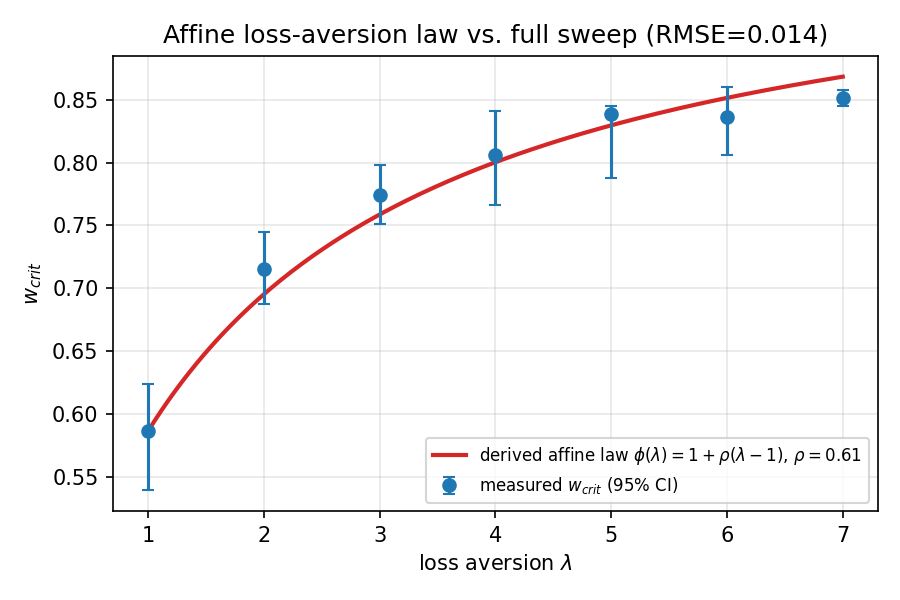
\includegraphics[width=0.82\columnwidth]{Figures/affine_law_7pt}
 \caption{The one-parameter saturating summary~\eqref{eq:wcrit_lambda} (line, one additional free
  parameter $\rho=0.61$ after anchoring $\gamma$ at $\lambda{=}1$) against measured $\wcrit(\lambda)$
  (points, bootstrap 95\% CIs). Held-out RMSE on $\lambda\in\{2,4,5,6\}$ is $0.016$; all-seven
  RMSE is $0.014$. The fit is an interpolation within one sweep, not out-of-distribution
  validation.}
 \label{fig:affine}
\end{figure}

\begin{table}[t]
\centering
\caption{Claim ledger for the mechanism. Each row separates modeled signs, measured evidence, and
fitted quantities.}
\label{tab:ledger}
{\setlength{\tabcolsep}{3pt}\small
\begin{tabular}{@{}p{0.30\columnwidth}p{0.62\columnwidth}@{}}
\toprule
Modeled/sign-level & supply-chain PPO: increasing $w$ raises escape SNR; increasing $\lambda$
lowers escape SNR; loss aversion raises $\wcrit$ \\
\addlinespace
Measured generally & sharp boundary; horizon slide; loss-aversion direction across SC, MPE, LBF \\
\addlinespace
Measured only on SC & curvature lowers $\wcrit$; affine law; directed-flow minority cascade \\
\addlinespace
Calibrated/fitted & absolute $\wcrit$; diffusion scale; $\gamma$; $\rho$ after baseline anchoring \\
\addlinespace
Future work & closed-form numerical $\wcrit$; universal curvature sign; affine-law transfer \\
\bottomrule
\end{tabular}}
\end{table}

% =======================================================================
\section{The Instrument Travels; So Does the Direction}
\label{sec:generalization}

The instrument is only useful if it can be measured beyond the supply chain. We estimate a CI'd
$\wcrit$ in four environment-algorithm combinations: the supply chain under MAPPO (changing only the
learner), and Cooperative Navigation (MPE) and Level-Based Foraging (LBF) under MAPPO (changing the
environment). The design is not fully crossed, because independent PPO floors out on the
shared-reward transfer tasks, so the supply-chain/MAPPO cell is what separates the learner change
from the environment change. In each we ask whether the loss-aversion direction travels; the
mechanism commits in advance to a sign through the SNR premise.

A transfer boundary is meaningful only if the learner can coordinate at high centralization.
Independent PPO fails this prerequisite on the shared-reward transfer tasks: on MPE it collapses at
\emph{every} $w$ (a coordination floor), and the same floor appears on LBF (Supplement), so the
boundary is right-censored beyond the feasible $w$-range rather than absent. Centralized-critic
MAPPO~\citep{yu2022surprising} recovers coordination and exposes an interior boundary. On \emph{MPE}
(Cooperative Navigation) the team objective is landmark coverage; because MPE has no native
local--global conflict, we construct one with a herding wrapper that adds a local reward for staying
near other agents, and we calibrate its scale so the no-transform boundary is interior
($\wcrit=0.74$)---otherwise there is no crossing to shift. The reported MPE $\wcrit$ is therefore a
property of our wrapper, not of MPE; the scale was fixed before the $\lambda$-sweep, not selected on
loss-aversion outcomes. A run is labeled collapsed when landmark occupancy (fraction of landmarks
covered, averaged over evaluation) falls below the pre-specified threshold $\theta=0.144$.

The loss-aversion direction transfers in every measured setting
(Figure~\ref{fig:generalization}, Table~\ref{tab:generalization}). We report each setting at its
largest $\lambda$ with an interior boundary estimate---$\lambda{=}7$ for the supply chain and MPE,
$\lambda{=}4$ for LBF, whose crossing saturates against the $w{=}1$ ceiling beyond that point---and
at the common moderate value $\lambda{=}3$ for a like-for-like comparison. On the \emph{supply chain
under MAPPO} (only the learner changes), $\wcrit$ rises $0.796\to0.889$, monotone from $\lambda{=}2$
and converging with PPO by $\lambda\!\geq\!4$; on \emph{MPE}, $\wcrit$ rises $0.78\to0.89$, a
$+0.158$ shift over the no-transform null at $\lambda{=}7$ ($+0.101$ at $\lambda{=}3$, matching the
supply chain's $+0.089$); on \emph{LBF}, $\wcrit$ rises $0.26\to0.83$ by $\lambda{=}4$. The secondary
structure does not transfer: on MPE the curvature-only shift is indistinguishable from zero
($+0.042$, CI spans zero), and on LBF curvature moves the boundary \emph{right} rather than left
while the supply-chain summary form misfits the sweep (RMSE $0.15$). The portable claim is the CI'd
boundary and the loss-aversion direction; absolute levels, curvature sign, and summary form are
substrate-specific.

\paragraph{Scope condition: action representation.}
On the supply-chain base-stock control, the boundary depends on how finely the scalar action is
discretized. A single-variable control isolates why: value-based learners (QMIX, IQL) on a
discretized $K{=}11$ shell give a flat, $w$-independent collapse rate, but PPO on the \emph{same}
$K{=}11$ shell also goes flat (Table~\ref{tab:ablation}), so it is coarse scalar discretization, not
the value-based paradigm, that erases the boundary. That the effect is specific to \emph{coarse}
discretization, not to discreteness itself, is shown by MPE, which is natively discrete in action
labels yet retains a boundary. We read the supply-chain result as coarse bins snapping the policy to
fixed attractor levels and suppressing near-boundary exploration; it is a scope condition of this
substrate's coarse action encoding rather than a general requirement of the instrument, and is
established here only at $K{=}11$ (whether finer bins recover the boundary is untested). Because
value-based learners show no measurable boundary here, whether the loss-aversion direction holds
under them is not well-posed and we claim nothing about it; both learners we do use (PPO and
centralized-critic MAPPO) are policy-gradient, so applicability to value-based learners is an open
scope question rather than a tested negative.

\begin{table}[t]
\centering
\caption{Action-representation ablation. The control (last row) changes only the action space
while holding the learner at PPO, isolating coarse discretization as what erases the boundary.}
\label{tab:ablation}
{\setlength{\tabcolsep}{5pt}\small
\begin{tabular}{lll}
\toprule
Learner & Action space & Boundary? \\
\midrule
PPO / MAPPO & continuous & yes \\
QMIX (centralized value) & discrete $K{=}11$ & no \\
IQL (independent value) & discrete $K{=}11$ & no \\
PPO (control) & discrete $K{=}11$ & \textbf{no} \\
\bottomrule
\end{tabular}}
\end{table}

\begin{figure}[t]
 \centering
 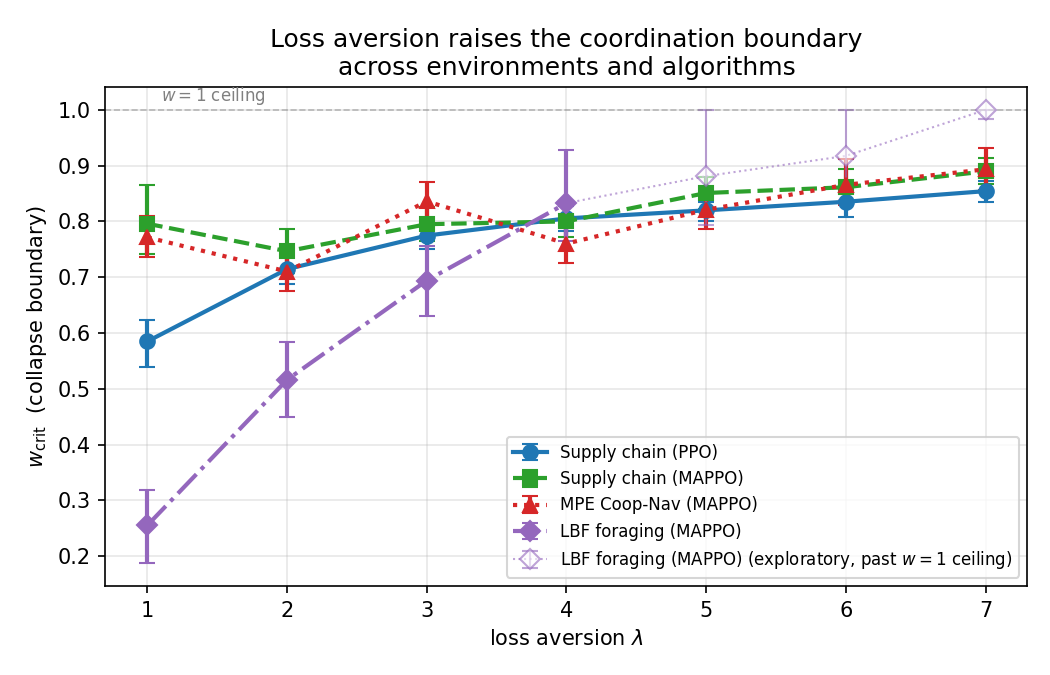
\includegraphics[width=0.95\columnwidth]{Figures/generalization_wcrit_vs_lambda.png}
 \caption{$\wcrit$ versus $\lambda$ across four settings: supply chain under PPO and MAPPO, MPE
  under MAPPO, LBF under MAPPO (bootstrap 95\% CIs). $\wcrit$ rises with $\lambda$ in every
  setting; the \emph{direction} generalizes, while levels (most at $\lambda{=}1$), curvature
  sign, and exact form are substrate-specific. LBF $\lambda{\geq}5$ points extrapolate past the
  $w{=}1$ ceiling (outside the measured grid) and are labeled exploratory.}
 \label{fig:generalization}
\end{figure}

\begin{table}[t]
\centering
\caption{Generalization of the loss-aversion \emph{direction}. Endpoints are within-sweep
($\alpha{=}\beta{=}0.88$), reported $\lambda{=}1\to7$ where both are interior; LBF uses its last
interior endpoint ($\lambda{=}4$). Parenthetical values are endpoint differences; shifts against
each setting's no-transform null appear in the text and Supplement.}
\label{tab:generalization}
\scriptsize
\begin{tabular}{p{0.28\columnwidth}p{0.34\columnwidth}p{0.18\columnwidth}}
\toprule
Setting (algo.) & Endpoints ($\lambda{=}1\to$last) & Summary form? \\
\midrule
Supply (PPO)  & $0.586\!\to\!0.852$ ($+0.266$) & yes \\
Supply (MAPPO) & $0.796\!\to\!0.889$ ($+0.093$) & -- \\
MPE (MAPPO) & $0.78\!\to\!0.89$ ($+0.11$) & no \\
LBF (MAPPO) & $0.26\!\to\!0.83$ ($+0.57$, by $\lambda{=}4$) & no (0.15) \\
\bottomrule
\end{tabular}
\end{table}

% =======================================================================
\section{A Single Downstream Node Can Nearly Set the Boundary}
\label{sec:minority}

This experiment is necessarily supply-chain-only: it requires a directed resource-flow topology
(a DAG) that MPE and LBF, as non-networked coordination tasks, do not have. The main sweep is
homogeneous, every trained node using the same $\lambda$; here we make one node loss-averse while
the others stay risk-neutral, holding the environment, PPO configuration, collapse label, $w$-grid,
and boundary estimator identical to the main sweep. We ask two questions: can one biased node move
the boundary by itself, and does its position determine the size of the shift
(Figure~\ref{fig:cascade})? Position could matter because the six-node network is a branching DAG:
demand enters at the retail edge, two downstream trained nodes feed demand most directly, and
upstream suppliers feed one or both downstream paths, so a loss-averse node should matter more when
its output reaches demand through a short, concentrated path. Because MPE and LBF lack this topology,
the cascade is a falsifiable prediction for any branching directed-flow domain---traffic networks,
power grids, multi-echelon logistics---that we state here and test only on the supply chain.

\paragraph{A single node, dose for dose.}
Sweeping the most downstream node's $\lambda\in\{1,\dots,7\}$ (others risk-neutral) traces a
strictly monotone dose-response: $\wcrit$ rises $0.586\to0.856$, converging on the \emph{fully}
loss-averse value ($0.852$) by $\lambda{=}7$ (Figure~\ref{fig:cascade}b). The single-node curve has
the same saturating shape as the homogeneous $\lambda$-sweep and shares its start and endpoint,
though its independent variable is one node's $\lambda$ rather than the team's; whether the two
curves coincide at intermediate $\lambda$---which would make the homogeneous law effectively this
node's law---is a question we flag but do not resolve here. Operationally, the team's collapse
boundary is not an average over agents: it is set, nearly entirely, by whichever node's output
reaches demand most directly, so an audit of reward transforms should target that node, not the
mean.

\paragraph{Position: proximity to demand, not chain index.}
Placing one $\lambda{=}7$ node at each position, the effect is strongly position-dependent, but the
governing variable is how directly a node's output reaches demand, not a chain index
(Figure~\ref{fig:cascade}a). The two nodes feeding retail directly dominate ($0.856$, $0.800$); the
upstream supplier feeding \emph{only} the dominant downstream node is nearly as strong ($0.797$),
while those \emph{splitting} output across both are weaker ($0.726$, $0.673$). The network is a
branching DAG, not a chain, and $\wcrit$ tracks a qualitative \emph{path concentration} pattern: a
biased node matters more the more directly and exclusively its product flows to demand. Where
\citet{mengesha2025} find loss aversion's effect on cooperation is \emph{non-monotone} in an
evolutionary model, the effect here is monotone in deep MARL and carries a topological signature,
which suggests the sign is a property of the dynamics rather than of the preference structure.

\begin{figure}[t]
 \centering
 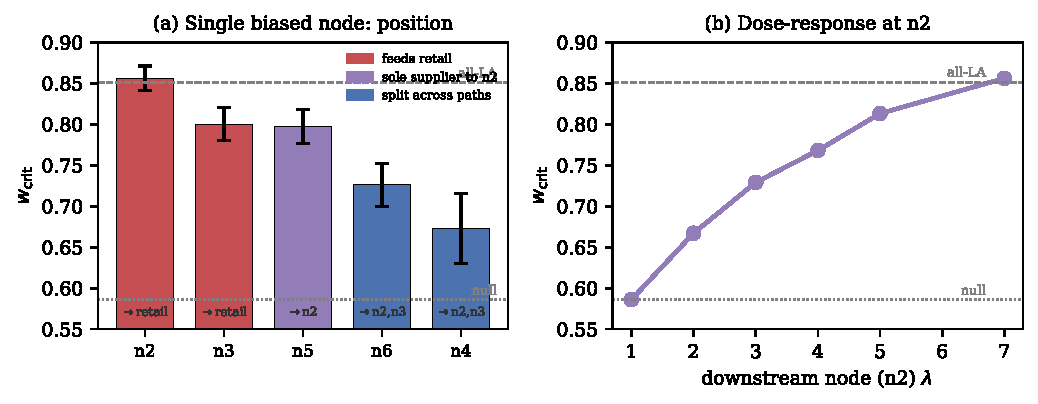
\includegraphics[width=\columnwidth]{Figures/cascade_tier_dose}
 \caption{A single loss-averse node can dominate the supply-chain boundary. (a)~One
  $\lambda{=}7$ node by position: the largest shifts come from nodes whose output reaches demand
  most directly, nodes feeding retail (red) dominate, the sole supplier to the dominant
  downstream node (purple) nearly matches them, and split-path suppliers (blue) are weaker.
  (b)~Dose-response: increasing the downstream node's $\lambda$ moves $\wcrit$ monotonically up
  to the homogeneous all-loss-averse value ($0.852$, dashed).}
 \label{fig:cascade}
\end{figure}

% =======================================================================
\section{Discussion}
\label{sec:discussion}

To our knowledge, no prior work separates the value transform's curvature and loss-aversion
components in cooperative MARL; prior work applies prospect theory as a unified
model~\citep{lalmohammed2025,ghaemi2024risk}. Decomposing it shows that on our primary substrate the
two components move the boundary in \emph{opposite} directions and would partially cancel if reported
jointly, so a single ``prospect-theoretic'' condition can under-report the loss-aversion effect by
about half. The curvature sign is substrate-specific (it does not transfer to MPE or LBF), but this
methodological point survives all three settings. The operational reading is concrete: a system of
$\lambda{=}7$ reward-transformed agents has a 50\% collapse midpoint at $w=0.852$ against $w=0.685$
for risk-neutral agents, a $+0.167$ margin that scales with $\lambda$. Our phase-diagram framing
sits within a recognized line of multiagent phase-transition
results~\citep{yamaguchi2025,capannoli2026phase} and the broader cooperative-AI
project~\citep{dafoe2020open,hammond2025multiagent,barfuss2020caring}; the distinctive
contribution is a measured reward-centralization boundary with a supporting signal-to-noise
account.

\paragraph{Operational interpretation.}
The boundary is a design quantity. A team can estimate its own $\wcrit$ and budget for the
loss-aversion margin rather than discover collapse in production: if architectural constraints cap
$w$ at, say, $0.8$, the usable loss-aversion budget is bounded by where $\wcrit$ crosses that cap,
about $\lambda\approx4$ on this substrate. Where $\lambda$ is not set by hand but induced by a reward
transform or training objective, it becomes a second lever to measure rather than
assume~\citep{ethayarajh2024kto,rabin2000risk}. The minority result adds a targeting rule: audit the
biased node whose output most directly reaches demand, not the average agent. This topology
information is dual-use---the same map that hardens the most influential node also identifies where
an induced bias would most degrade coordination---which we address in the ethics statement.

\paragraph{Scope and Future Work.}
Three limits each point to a concrete next step. First, the quantitative core (the $\wcrit(\lambda)$
summary and the cascade) is single-substrate by construction: the direction, boundary, and
metastable slide replicate across the four measured environment-algorithm combinations, but the
magnitudes belong to one simulator and the summary form does not transfer to MPE or LBF. Replicating
the cascade on a second directed-flow domain would make it a tested generalization. Second, the
mechanism fixes sign and form but not magnitude; localizing $\wcrit$ from the learning dynamics
resisted two pre-committed probes, both of which track \emph{where the policy sits}, not \emph{where
the boundary is} (Supplement), so a localizing observable that predicts $\wcrit$ without a full sweep
is the clearest open problem. Third, our $\lambda$ is set by hand; in deployed preference-aligned
systems $\lambda$ is induced by the training objective and its effective value is unknown, so
estimating it from behavior would connect the reward-transform axis to real training pipelines.

% =======================================================================
\section{Conclusion}
\label{sec:conclusion}

Reward centralization is usually treated as a direction: more team signal helps. We have shown that
it also has a measurable location---a critical fraction $\wcrit$ that a team can estimate on its own
system with confidence intervals of a few hundredths---and that this location moves: rightward under
loss-averse reward transforms, leftward with a longer training horizon, and, on a directed supply
network, largely with the reward design of the downstream node nearest demand. The direction and the
horizon slide generalize across the four measured environment-algorithm combinations; the numerical
thresholds are specific to the systems we study, but the measurement protocol is not.

% =======================================================================
\section*{Ethical Statement}

This work is entirely simulated, with no human subjects or personal data. Reported thresholds are
substrate-specific and must be re-measured before operational use; the minority-node result is
dual-use (hardening versus targeted disruption) and reported explicitly for auditability.

% =======================================================================
\bibliography{references}

\end{document}
